%%%%%%%%%%%%%%%%%%%%%%%%%%%%%%%%%%%%%%%%%%%%%%%%%%%%%%%%%%%%%%%%%%%%%%%%%%%%%%%%
%
% 2.1.3: Delta-Sigma Linear System Models
%
%%%%%%%%%%%%%%%%%%%%%%%%%%%%%%%%%%%%%%%%%%%%%%%%%%%%%%%%%%%%%%%%%%%%%%%%%%%%%%%%

In order to ease the analysis and design of $\Delta\Sigma$ modulators, we generally
linearize the system by modeling the quantizer as an additive white noise source. This
linearized quantizer model is illustrated in Figure \ref{fig:linear_quantizer_model}
\cite{hayes_schaums_1998}.
%-------------------
\begin{figure}[htb]
 \centering
 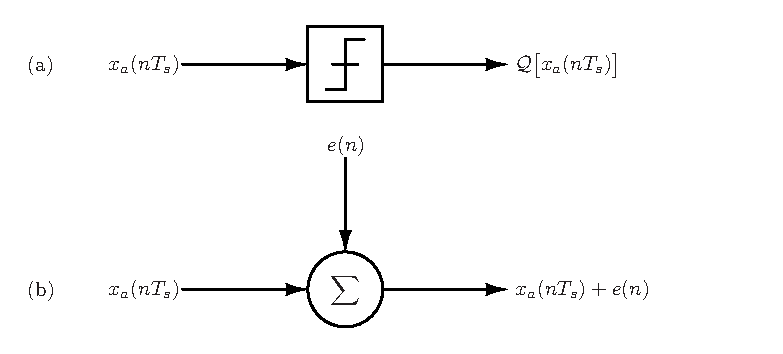
\includegraphics{./final_figures/linear_quantizer_model.eps}
 \caption{Linearized Quantizer Model}
 \label{fig:linear_quantizer_model}
\end{figure}
%-------------------
Substituting this linearized quantizer model into Figure \ref{fig:loop_filter_1}, we
arrive at the generalized hardware structure illustrated in Figure
\ref{fig:loop_filter_sum_noise}.
%-------------------
\begin{figure}[htb]
 \centering
 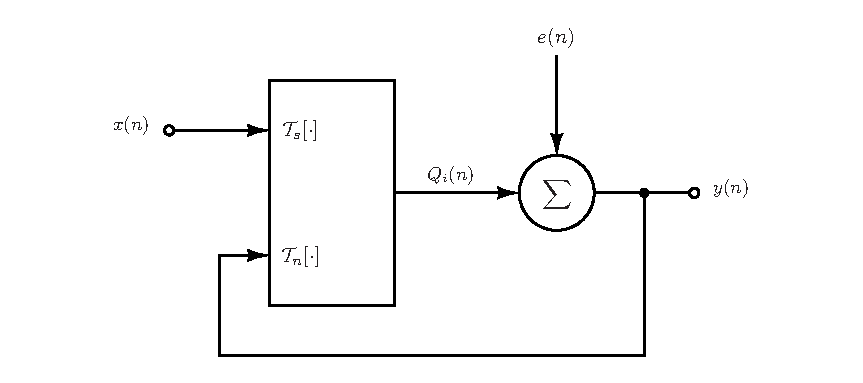
\includegraphics{./final_figures/loop_filter_sum_noise.eps}
 \caption{Linearized \DSm System Model}
 \label{fig:loop_filter_sum_noise}
\end{figure}
%-------------------
The following sections will present examples of first, second, and
generalized \nth \space order linear models of \DSms. 

%%%%%%%%%%%%%%%%%%%%%%%%%%%%%%%%%%%%%%%%%%%%%%%%%%%%%%%%%%%%%%%%%%%%%%%%%%%%%%%%
\subsubsection{First Order System}
The trivial case is offered by the first-order system. While impractical for
implementation, it offers a basis upon which to introduce the structural characteristics
of higher order devices. Figure \ref{fig:ct_first_order} illustrates a first-order \ct
system where $\hat{x}(t)$ denotes the \ct variable.
%-------------------
\begin{figure}[htbp]
 \centering
 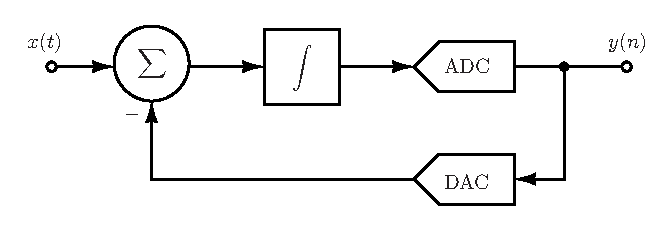
\includegraphics{./final_figures/ct_dsm_model.eps}
 \caption{First-Order \CTDSM}
 \label{fig:ct_first_order}
\end{figure}
%-------------------
Inspection of Figure \ref{fig:ct_first_order} yields two important characteristics: (1)
the back-end of the \DSm is discrete in nature (2) the system operation is driven by
accumulated error as function of time. Since the back-end of the \DSm is discrete
in nature, system design is often approached from the \dt
perspective\cite{hayes_schaums_1998}. However, \ct design methodologies are gaining
popularity as design complexities associated with realizing high-bandwidth switched
capacitor hardware increase \cite{cherry_continuous-time_1999}.

Figure \ref{fig:linear_z_model_1} illustrates a 1\textsuperscript{st} order \dt \DSm.
Note that the relevant signals are expressed as their $z$-transform equivalents
reflecting frequency domain analysis.
%-------------------
\begin{figure}[htbp]
 \centering
 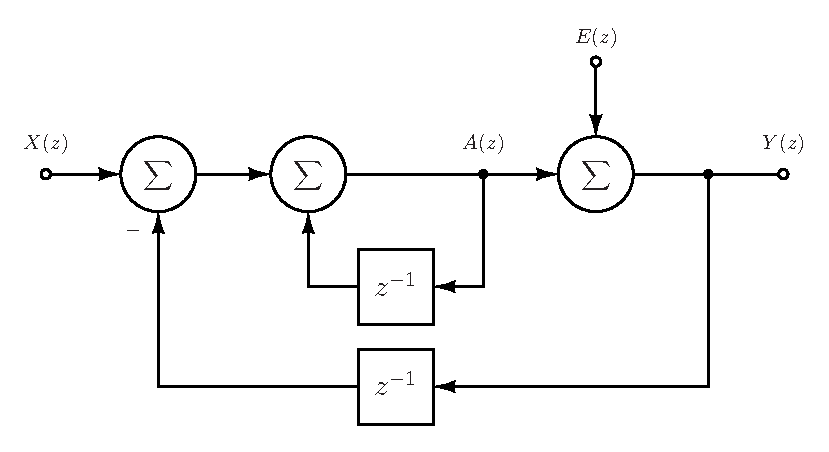
\includegraphics{./final_figures/first_order_simple.eps}
 \caption{1\textsuperscript{st} Order Linear Model}
 \label{fig:linear_z_model_1}
\end{figure}
%-------------------
Solving for the output, $Y(z)$, in Figure \ref{fig:linear_z_model_1} yields the
following
relationship.
%-------------------
\begin{equation}\label{eq:1st_lin_easy1}
 Y(z)=E(z)+A(z)
\end{equation}
%-------------------
Similarly, solving for the accumulator output, $A(z)$, in Figure
\ref{fig:linear_z_model_1} yields the following
equation.
%-------------------
\begin{equation}\label{eq:1st_lin_easy2}
 A(z)=z^{-1}A(z)+X(z)-z^{-1}Y(z)
\end{equation}
%-------------------
Substituting \eqref{eq:1st_lin_easy2} into \eqref{eq:1st_lin_easy1} yields the following
equation.
%-------------------
\begin{equation}\label{eq:1st_lin_easy3}
 \begin{split}
  Y(z) &= E(z)+z^{-1}A(z)+X(z)-z^{-1}Y(z)\\
       &= X(z)+E(z)-z^{-1}\bigl(Y(z)-A(z)\bigr)\\
       &= X(z)+\bigl(1-z^{-1}\bigr)E(z)
 \end{split}
\end{equation}
%-------------------
Observe that the coefficients for $X(z)$ and $E(z)$ represent the STF and the NTF
respectively. Specifically, these functions are given by the following expressions.
%-------------------
\begin{equation}\label{eq:first_order_STF_NTF}
  \begin{split} 
   \textrm{STF}(z)&=1\\
   \textrm{NTF}(z)&=\bigl(1-z^{-1}\bigr)
  \end{split}
\end{equation}
%-------------------
Finally, substituting \eqref{eq:first_order_STF_NTF} into \eqref{eq:1st_lin_3}
yields the following general expression. Note that this is identical to the
expression provided in \eqref{eq:DSM_output_1} where the signal and noise shaping
transformations correspond to the STF and NTF respectively.
\begin{equation}\label{eq:general_DSM_z_form}
 Y(z) = STF(z)X(z)+NTF(z)E(z)
\end{equation}

Note that the input signal, $X(z)$, is unaltered (unity gain) and the noise, $E(z)$, is
low-pass filtered by the single pole expression given in \eqref{eq:first_order_STF_NTF}.
Again, this trivial first order example has little practical application and only serves
to illustrate the basic functional structure.

%%%%%%%%%%%%%%%%%%%%%%%%%%%%%%%%%%%%%%%%%%%%%%%%%%%%%%%%%%%%%%%%%%%%%%%%%%%%%%%%
%%% Complex First-Order Model
In order to tune the operational region, we will need to provide coefficients respective
of the desired frequency response characteristics. This degree of freedom is the design
mechanism which enables the noise shaping to occur. This is illustrated in Figure
\ref{fig:linear_z_model_2}.
%-------------------
\begin{figure}[htbp]
 \centering
 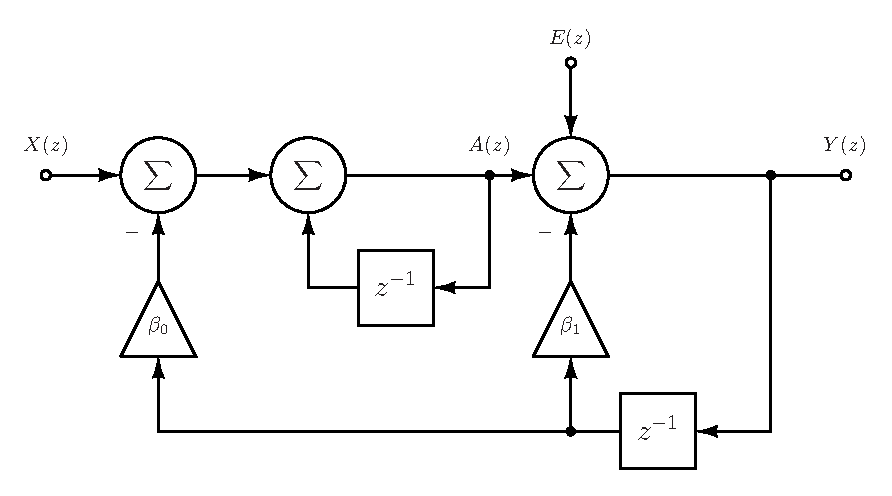
\includegraphics{./final_figures/first_order_linear_model.eps}
 \caption{Generalized First Order Linear Model}
 \label{fig:linear_z_model_2}
\end{figure}
%-------------------
Solving for the output, $Y(z)$, in Figure \ref{fig:linear_z_model_2} yields the
following relationship.
%-------------------
\begin{equation}\label{eq:1st_lin_1}
 Y(z)=E(z)+A(z)-\beta_{1}z^{-1}Y(z)
\end{equation}
%-------------------
Similarly, solving for $A(z)$ in Figure \ref{fig:linear_z_model_2} yields the following
equation.
%-------------------
\begin{equation}\label{eq:1st_lin_2}
 \begin{split}
 A(z) &= z^{-1}A(z)+X(z)-\beta_{0}z^{-1}Y(z)\\
      &= \frac{X(z)-\beta_{0}z^{-1}Y(z)}{\bigl(1-z^{-1}\bigr)}
 \end{split}
\end{equation}
%-------------------
Substituting \eqref{eq:1st_lin_2} into \eqref{eq:1st_lin_1} yields the following
equation.
%-------------------
\begin{equation}\label{eq:1st_lin_3}
  \begin{split}
  Y(z) &= E(z)+z^{-1}A(z)+X(z)-\beta_{0}z^{-1}Y(z)-\beta_{1}z^{-1}Y(z)\\
      &=
\frac{\bigl(1-z^{-1}\bigr)E(z)+X(z)}{\Bigl(1+\bigl(\beta_{0}+\beta_{1}-1\bigr)z^{-1}
-\beta_{1}z^{-2}\Bigr)}\\
     &= \frac{X(z)}{\Bigl(1+\bigl(\beta_{0}+\beta_{1}-1\bigr)z^
 {-1}-\beta_{1}z^{-2}\Bigr)}+\frac{\bigl(1-z^{-1}\bigr)E(z)}{\Bigl(1+\bigl(\beta_{0}
 +\beta_{1}-1\bigr)z^{-1}-\beta_{1}z^{-2}\Bigr)}
 \end{split}
\end{equation}
%-------------------
Similar to expression \eqref{eq:first_order_STF_NTF}, we can show the following.
%-------------------
\begin{equation}\label{eq:1st_lin_4}
 \begin{split}
   \textrm{STF}(z)&=
	\frac{1}{\Bigl(1+\bigl(\beta_{0}+\beta_{1}-1\bigr)z^{-1}-\beta_{1}z^{-2}\Bigr)}\\
 \textrm{NTF}(z)&=
	\frac{\bigl(1-z^{-1}\bigr)}{\Bigl(1+\bigl(\beta_{0}+\beta_{1}-1\bigr)z^{-1}-
	\beta_{1}z^{-2}\Bigr)}
 \end{split}
\end{equation}
%-------------------

Clearly these results are more complex than the equations derived for the trivial
1\textsuperscript{st} order case. However, $\beta_1$ is typically set to zero and is only
included here for completeness. Further, setting $\beta_0=1$ and solving for
the output results in the expressions given in \eqref{eq:1st_lin_easy3}. Substituting
$n=1$ into \eqref{eq:peak_SNR_with_NTF} yields a marked improvement over performance
without noise shaping. However, it is still insufficient for practical applications. Thus,
a detailed example of a usable 2\textsuperscript{nd} order system is provided in the
following section.

%%%%%%%%%%%%%%%%%%%%%%%%%%%%%%%%%%%%%%%%%%%%%%%%%%%%%%%%%%%%%%%%%%%%%%%%%%%%%%%%
\subsubsection{2nd Order System}
While the first order system is of academic interest, it is of little
practical value. Here we will present a second order system. Note that the
second order system is created by cascading two first order systems
together as illustrated in Figure \ref{fig:linear_z_model_2nd_order}.
%-------------------
\begin{figure}
  \centering
  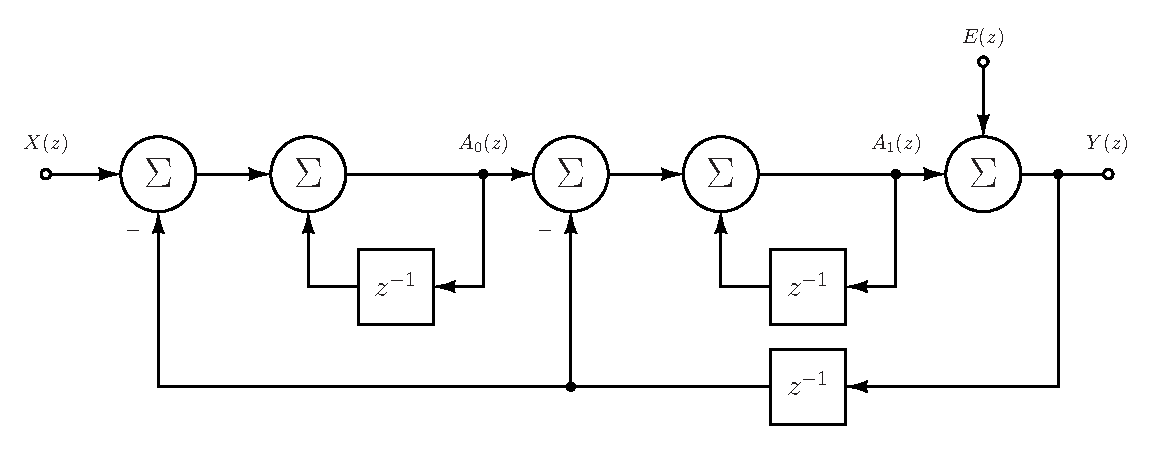
\includegraphics[width=\textwidth]{./final_figures/second_order_simple_model.eps}
  \caption{Second Order Linear Model}
  \label{fig:linear_z_model_2nd_order}
\end{figure}
%-------------------
Solving for the accumulator outputs, denoted $A_{0}$ and $A_{1}$, yields the following
equations.
%-------------------
\begin{equation}\label{eq:2nd_order_DSM_accumulators}
  A_{0}(z) = \frac{X(z)-z^{-1}Y(z)}{1-z^{-1}} ,\quad
  A_{1}(z) = \frac{A_{0}(z)-z^{-1}Y(z)}{1-z^{-1}}
\end{equation}
%-------------------
Finally, solving for the output $Y(z)$ in terms of \eqref{eq:2nd_order_DSM_accumulators}
yields the following expression.
%-------------------
\begin{equation}\label{eq:2nd_order_DSM_output}
 \begin{split}
  Y(z) &= E(z)+A_1(z) \\
       &= X(z)+ \bigl(1-z^{-1}\bigr)^2 E(z)
 \end{split}
\end{equation}
%-------------------

As done previously, we will generalize the form of the structure to include
coefficients for tuning the shape of the noise transfer function. Figure
\ref{fig:linear_z_model_2nd_order_complex} illustrates a more complex second
order system. Note that the accumulator loop has been condensed into a single block
for ease of analysis and illustration.
%-------------------
\begin{figure}
  \centering
  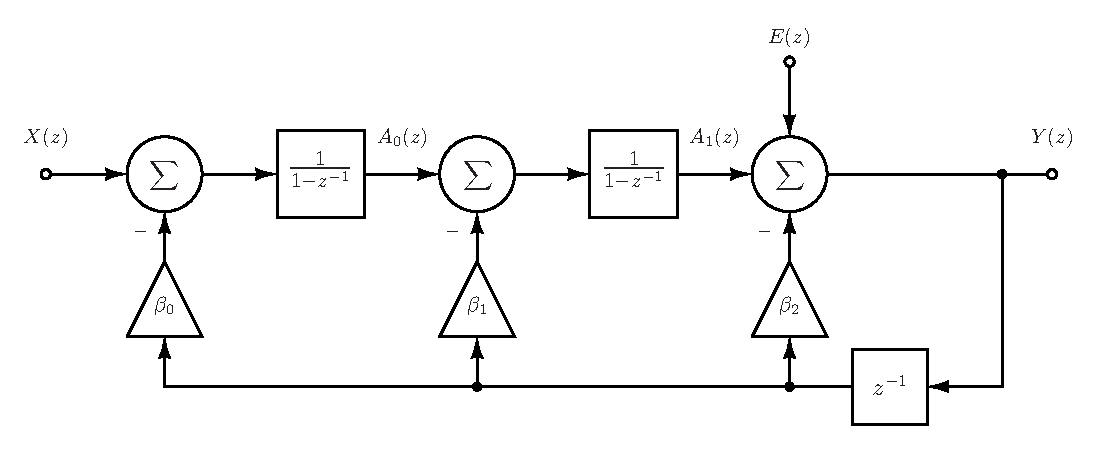
\includegraphics[width=\textwidth]{./final_figures/second_order_complex_model.eps}
  \caption{Generalized Second Order Linear Model}
  \label{fig:linear_z_model_2nd_order_complex}
\end{figure}
%-------------------
Again, solving for the accumulator outputs, denoted $A_{0}$ and $A_{1}$, yields
the following equations.
%-------------------
\begin{equation}\label{eq:2nd_order_DSM_accumulators_complex}
  A_{0}(z) = \frac{X(z)-\beta_0 z^{-1}Y(z)}{1-z^{-1}} ,\quad
  A_{1}(z) = \frac{A_{0}(z)-\beta_1 z^{-1}Y(z)}{1-z^{-1}}
\end{equation}
%-------------------
Solving for the output $Y(z)$ in terms of
\eqref{eq:2nd_order_DSM_accumulators_complex} yields the following expression.
%-------------------
\begin{equation}\label{eq:2nd_order_DSM_output_complex}
 \begin{split}
  Y(z) &= E(z)+A_1(z)-\beta_2 z^{-1}Y(z) \\
       &= \frac{X(z)+ \bigl(1-z^{-1}\bigr)^2 E(z)}
{ 1+ z^{-1}\bigl(-2+\beta_0+\beta_1+\beta_2\bigr)
   + z^{-2}\bigl(1-\beta_1-2\beta_2\bigr)
   + z^{-3}\beta_2}\\
       &= \frac{X(z)}{
  1+ z^{-1}\bigl(-2+\beta_0+\beta_1+\beta_2\bigr)
   + z^{-2}\bigl(1-\beta_1-2\beta_2\bigr)
   + z^{-3}\beta_2}\\ 
       &\quad + \frac{\bigl(1-z^{-1}\bigr)^2 E(z)}{
  1+ z^{-1}\bigl(-2+\beta_0+\beta_1+\beta_2\bigr)
   + z^{-2}\bigl(1-\beta_1-2\beta_2\bigr)
   + z^{-3}\beta_2}
 \end{split}
\end{equation}
%-------------------
As with the first order case, $\beta_2$ is typically zero simplifying the
expression in \eqref{eq:2nd_order_DSM_output_complex} slightly. Observe that the
introduction of additional coefficients in the feedback loop allows the designer to tune
the pole locations for the NTF. This capability will prove critical in optimizing the
design of the NTF.

Often, the STF is largely ignored or assumed to be unity in \DSm design. This is due to
the fact that the in-band behavior of the STF must preserve unity gain by definition. 
However, it is trivial to introduce feedforward coefficients into the structure shown in
\ref{fig:linear_z_model_2nd_order_complex} as illustrated by Figure
\ref{fig:general_2nd_order}.
%-------------------
\begin{figure}
  \centering
  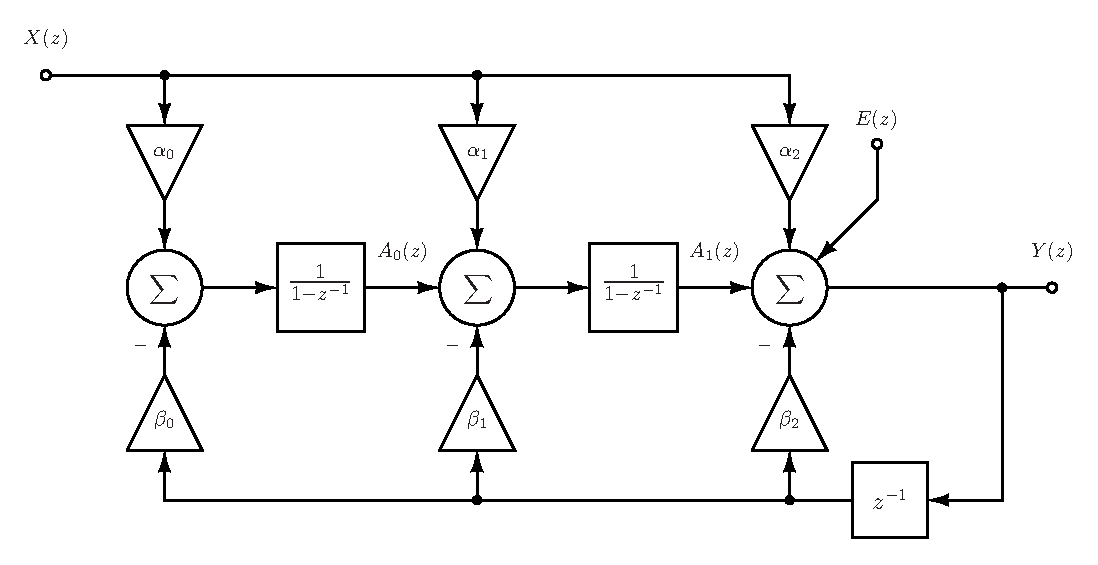
\includegraphics[width=\textwidth]{./final_figures/general_2nd_order.eps}
  \caption{Generalized Second Order Linear Model with Feedforward Coefficients}
  \label{fig:general_2nd_order}
\end{figure}
%-------------------
Solving for the accumulator outputs, denoted $A_{0}$ and $A_{1}$, yields
the following equations.
%-------------------
\begin{equation}\label{eq:2nd_order_DSM_accumulators_general}
  A_{0}(z) = \frac{\alpha_0 X(z)-\beta_0 z^{-1}Y(z)}{1-z^{-1}} ,\quad
  A_{1}(z) = \frac{\alpha_1 X(z)+ A_{0}(z)-\beta_1 z^{-1}Y(z)}{1-z^{-1}}
\end{equation}
%-------------------
Similarly, solving for the output $Y(z)$ yields the following expression.
%-------------------
\begin{equation}\label{eq:2nd_order_DSM_output_general}
 Y(z)=E(z)+\alpha_2 X(z)+A_1(z)-\beta_2 z^{-1}Y(z)
\end{equation}
%-------------------
Substituting \eqref{eq:2nd_order_DSM_accumulators_general} into
\eqref{eq:2nd_order_DSM_output_general} and simplifying produces the following expression.
%-------------------
\begin{equation}\label{eq:2nd_order_DSM_output_general_2}
\begin{split}
 Y(z)&=\left(\frac{
\bigl(\alpha_0+\alpha_1+\alpha_2\bigr)+\bigl(-\alpha_1+2\alpha_2\bigr)z^{-1}+\alpha_2
z^{-2}}
{\bigl(1+\beta_0+\beta_1\bigr)+\bigl(-2+\beta_1+\beta_2\bigr)z^{-1}+\bigl(1-2\beta_2\bigr)
z^{-2}+\beta_2z^{-3}}\right) X(z)\\
&\quad + \left(\frac{\bigl(1-z^{-1}\bigr)^2}
 {\bigl(1+\beta_0+\beta_1\bigr)+\bigl(-2+\beta_1+\beta_2\bigr)z^{-1}
+\bigl(1-2\beta_2\bigr)
z^{-2}+\beta_2z^{-3}}\right)E(z) 
\end{split}
\end{equation}
%-------------------
It is clear on inspection of \eqref{eq:2nd_order_DSM_output_general_2} that careful
selection of the feedback and feedforward coefficients allows the system designer to
control the pole and zero locations of the signal and noise transfer functions. This
degree of design freedom allows the designer to custom tune the functions to very specific
design requirements. This will be illustrated in the following chapter.

% %%%%%%%%%%%%%%%%%%%%%%%%%%%%%%%%%%%%%%%%%%%%%%%%%%%%%%%%%%%%%%%%%%%%%%%%%%%%%%%%
\subsubsection{Nth Order System}
The structure illustrated in Figure \ref{fig:general_2nd_order} offers a second
order case where the designer is free to select feedforward and feedback coefficients. In
practice, the designer will also place scaling coefficients between adjacent integrator stages.
Note that finite power supply limitations govern the hardware implementation of these devices.
Exceeding the bounds set by the power supply results in saturation of the stage where
it occurs. Great care must be taken to prevent this from occurring as it introduces
nonlinear distortion thereby decreasing the overall SNR. Figure
\ref{fig:linear_z_model_nth_order} illustrates a generalized \nth \space order converter
topology with these scaling coefficients between adjacent integrator stages.

%-------------------
\begin{sidewaysfigure}[htbp]
  \centering
  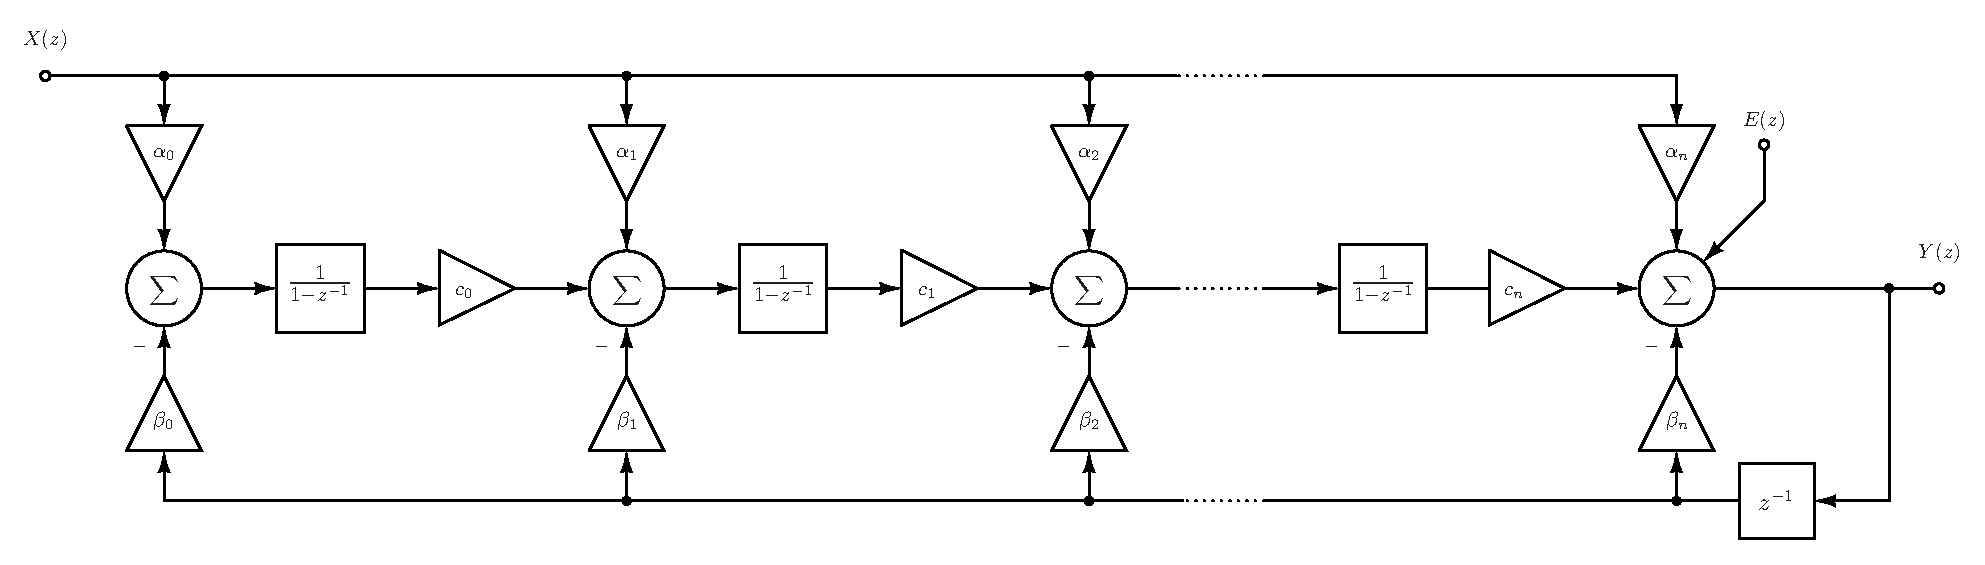
\includegraphics[width=\textwidth]{./final_figures/general_nth_order_2.eps}
  \caption{Generalized Nth Order Linear Model}
  \label{fig:linear_z_model_nth_order}
\end{sidewaysfigure}
%-------------------

Theoretically, the order of the system has no upper bound. However, the order of the
system rarely exceeds 8 for practical applications. Orders above that would suggest SNR values 
which are physically unrealizable in contemporary process technology. In addition, the level of system 
design complexity is directly proportional to the order of the system. Once non-ideal limitations are 
addressed, the acceptable tolerance becomes prohibitive for high order systems.  Thus, only systems of order 8 or less will be considered here. 

So far, only low-pass systems have been discussed. Certain applications require the operational region to be higher in frequency than flicker noise. This is achieved through a bandpass configuration. The bandpass configuration is achieved by by introducing recursion into the structure shown in \ref{fig:linear_z_model_nth_order}. This feedback path creates a resonator
and the topology is referred to as a cascade of resonators feedback (CRFB) system. Note, however, that the bandpass implementation effectively doubles the order of the system by placing frequency response constraints on the system which may or may not impact the overall system performance.